\section{Alpine}

We refer to an alpine climate, here, as one that sees below zero temperatures during a given period of the year. These extreme temperatures ensure only plant species able to survive in sub-zero temperatures survive in the long term. It is possible, however, for annuals to sprout during periods when the temperature increases.\\

\subsection{Resource Configuration}

Verbier, a Swiss alpine city at a latitude of 43\textdegree south, is the location on which climate data is
based for these tests.\\

To model a dry loamy soil, the soil infiltration rate is set to ten millimetres per hour (see figure \ref{tab:soil_types}). To
model rocky cliff faces, the soil infiltration rate is set to zero when the slope angle surpasses forty-five degrees.\\

The configured monthly rainfall and rainfall intensity are summarized in figure \ref{fig:results_alpine_input}. The resulting water build-ups and networks that form on the terrain are illustrated in figure \ref{fig:results_alpine_water_networks}.\\

The temperature extremes configured are thirty degrees for June and zero degrees for December with, resulting in monthly temperatures outlined in figure \ref{fig:results_alpine_input}. To more accurately represent the drastic change in temperature that occurs in alpine climates, the lapse rate is set to a ten degree drop in temperature for every thousand metres of altitude gained.\\

\begin{figure}
\center
	\includegraphics[width=\textwidth]{results_alpine_input.png}
	\caption{ \textit{Alpine: Input resource configurations: Rainfall (top-left), rainfall intensity (top-right) and temperature (bottom).}}
	\label{fig:results_alpine_input}
\end{figure}

\begin{figure}
\center
	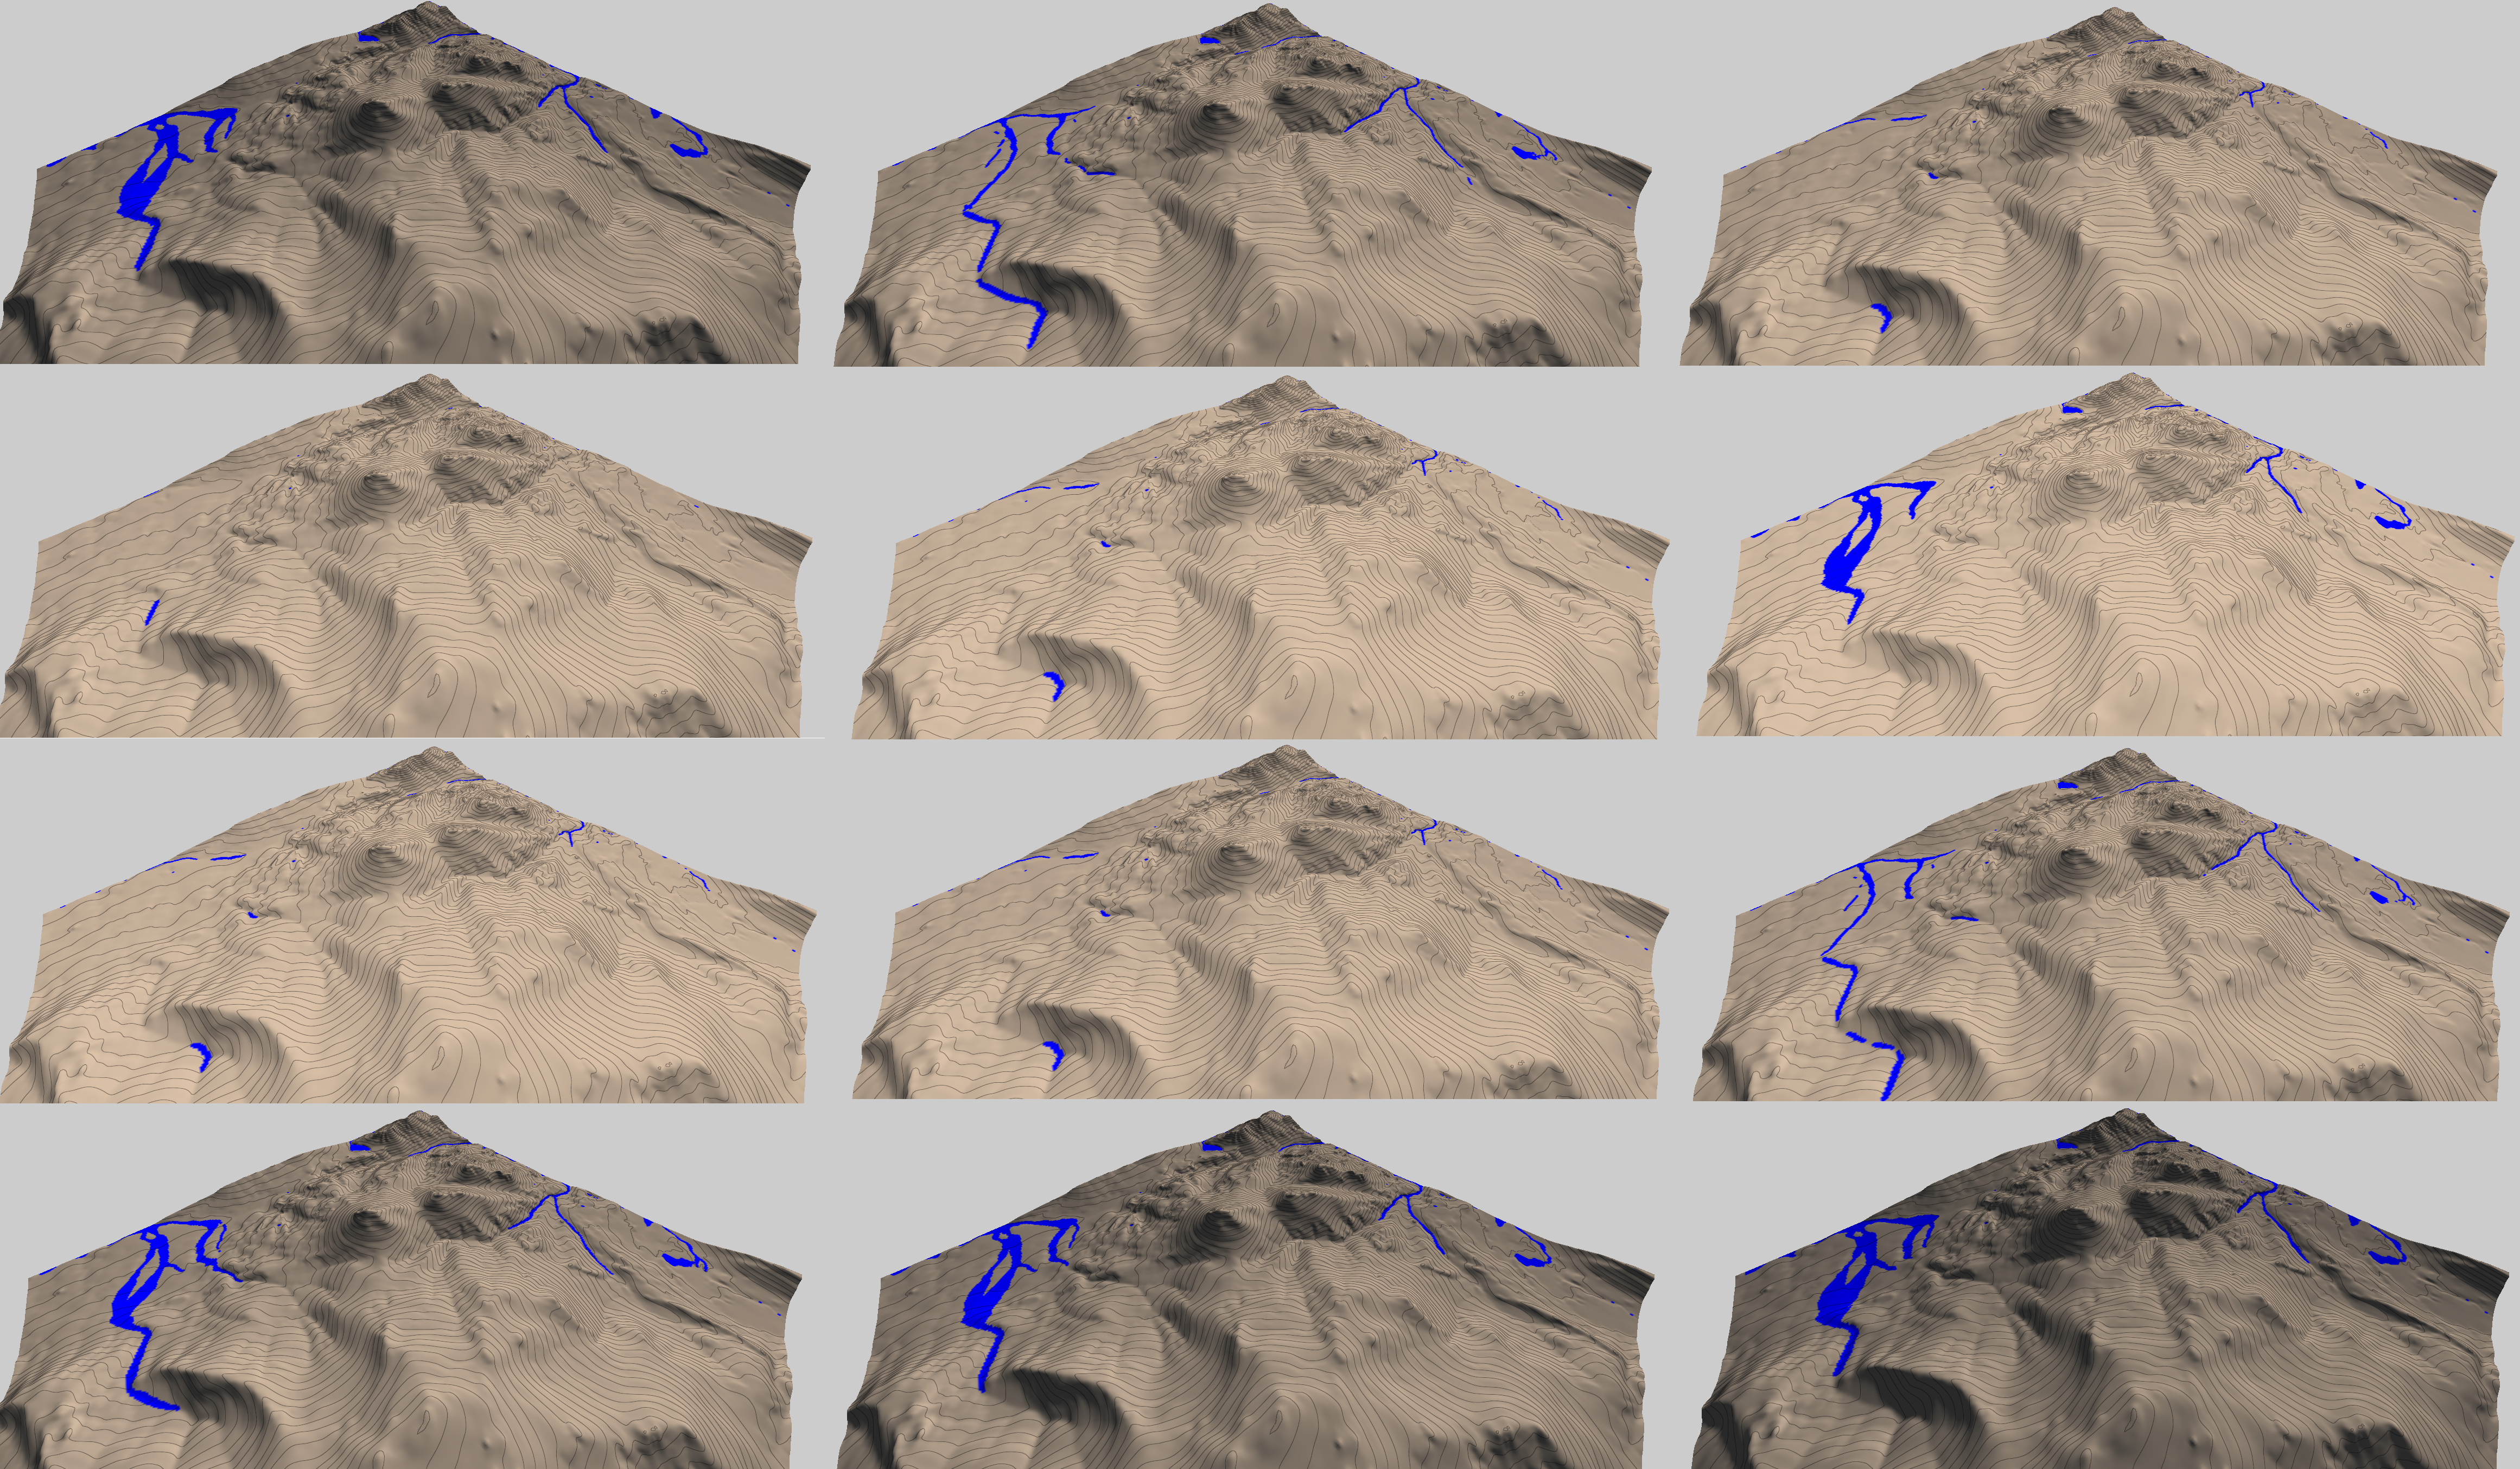
\includegraphics[width=\textwidth]{results_alpine_water_networks.png}
	\caption{\textit{Alpine: Water networks that form on the terrain at every month. From left to right, top to bottom.}}
	\label{fig:results_alpine_water_networks}
\end{figure}

\subsection{Clusters}

The number of clusters to generate is set to ten. The clustered terrain is shown in figure \ref{fig:results_alpine_terrain_clusters} and the corresponding cluster properties summarized in figure \ref{fig:results_alpine_cluster_hum_temp_illum} and table \ref{tab:results_alpine_cluster_slope_covarea}. 

\begin{figure}
\center
	\includegraphics[width=\textwidth]{results_alpine_clusters_on_terrain.png}
	\caption{\textit{Alpine: Resulting terrain clusters. Refer to table \ref{tab:results_alpine_cluster_slope_covarea} for cluster ID to cluster colour relationships.}}
	\label{fig:results_alpine_terrain_clusters}
\end{figure}

\begin{figure}
\center
	\includegraphics[width=\textwidth]{results_alpine_clusters_hum_illum_temp.png}
	\caption{\textit{Alpine: Cluster illuminations (top-left), soil humidities (top-right) and temperatures (bottom) for each terrain cluster with color coding to match that of the cluster overlay in figure \ref{fig:results_alpine_terrain_clusters}. Note that soil humidity data is removed for cluster 4 because the values are too large.}}
	\label{fig:results_alpine_cluster_hum_temp_illum}
\end{figure}

\definecolor{alpine_cluster_1}{rgb}{0.8,0.4,0.0}
\definecolor{alpine_cluster_2}{rgb}{0.6,0.4,0.4}
\definecolor{alpine_cluster_3}{rgb}{0.0,0.2,0.4}
\definecolor{alpine_cluster_4}{rgb}{1.0,1.0,0.4}
\definecolor{alpine_cluster_5}{rgb}{0.0,0.6,1.0}
\definecolor{alpine_cluster_6}{rgb}{1.0,0.0,0.0}
\definecolor{alpine_cluster_7}{rgb}{0.8,0.2,0.0}
\definecolor{alpine_cluster_8}{rgb}{1.0,0.4,0.8}
\definecolor{alpine_cluster_9}{rgb}{0.0,0.8,0.4}
\definecolor{alpine_cluster_10}{rgb}{0.8,0.4,1.0}

\begin{table}[h]
  \centering
	    \begin{tabular}{|p{5cm}|p{5cm}|p{5cm}|}
		\hline	
  	    \textbf{Cluster ID} & \textbf{Slope (degrees)} & \textbf{Coverage area (\% of terrain)} \\
  	    \hline	
		\cellcolor{alpine_cluster_1} 1 & 10.2 & 18 \\
		\hline
		\cellcolor{alpine_cluster_2} 2 & 21.1 & 13.5 \\
		\hline
		\cellcolor{alpine_cluster_3} 3 & 35.8 & 3.7 \\
		\hline
		\cellcolor{alpine_cluster_4}4 & 5.3 & 2 \\
		\hline
		\cellcolor{alpine_cluster_5} 5 & 19.9 & 4.2 \\
		\hline
		\cellcolor{alpine_cluster_6} 6 & 22.3 & 10.4 \\
		\hline
		\cellcolor{alpine_cluster_7} 7 & 28.2 & 9.3 \\
		\hline
		\cellcolor{alpine_cluster_8} 8 & 5 & 15 \\
		\hline
		\cellcolor{alpine_cluster_9} 9 & 15.7 & 19.4 \\
		\hline
		\cellcolor{alpine_cluster_10} 10 & 28.7 & 4.2 \\
		\hline
		\end{tabular}
		\caption{Alpine: Cluster slope and coverage area with color coding matching the cluster overlay in figure \ref{fig:results_tropical_terrain_clusters}.}
	  \label{tab:results_alpine_cluster_slope_covarea}
\end{table}


\subsection{Vegetation}

Five alpine plant species are configured for this test: \textit{Spruce}, \textit{Maple}, \textit{Lichen}, \textit{Daisy} and \textit{Beech}. The properties associated with each are summarized in appendix \ref{AppendixF}.\\

Tables \ref{tab:results_alpine_species_suitability} summarizes the species suitability to each calculated cluster. From this, it is possible to conclude that no plants are able to grow, and therefore no ecosystem simulator needs to be run, for cluster 4. This is caused by an excess in humidity as this cluster represents areas on the terrain covered in water.\\ 
This data also shows that Daisies are only suited to grow in cluster 8. In all other clusters, the temperature drops below its minimum. \\

\definecolor{color_red}{rgb}{1.0,0.0,0.0}
\definecolor{color_green}{rgb}{0.0,1.0,0.0}
\definecolor{color_orange}{rgb}{1.0,0.65,0.0}

\begin{table}[h]
  \centering
	    \begin{tabular}{|p{2cm}|p{2.5cm}|p{2.5cm}|p{2.5cm}|p{2.5cm}|p{2.5cm}|}
		\hline	
		&  \textbf{Spruce} & \textbf{Maple} & \textbf{Lichen} & \textbf{Daisy} & \textbf{Beech}\\
		\hline	
		Cluster 1 & 
		Y & 
		Y & 
		Y & 
		\cellcolor{color_red}N (T$^{-}$) & 
		Y \\
		\hline	
		Cluster 2 & 
		Y & 
		Y & 
		Y & 
		\cellcolor{color_red}N (T$^{-}$) & 
		Y \\
		\hline	
		Cluster 3 & 
		\cellcolor{color_red}N (S$^{+}$) & 
		Y & 
		Y & 
		\cellcolor{color_red}N (T$^{-}$) & 
		Y \\
		\hline	
		Cluster 4 & 
		\cellcolor{color_red}N (SH$^{+}$) & 
		\cellcolor{color_red}N (SH$^{+}$) & 
		\cellcolor{color_red}N (SH$^{+}$) & 
		\cellcolor{color_red}N (SH$^{+}$) & 
		\cellcolor{color_red}N (SH$^{+}$) \\
		\hline	
		Cluster 5 & 
		Y & 
		Y & 
		Y & 
		\cellcolor{color_red}N (T$^{-}$) & 
		Y \\
		\hline	
		Cluster 6 & 
		Y & 
		Y & 
		Y & 
		\cellcolor{color_red}N (T$^{-}$) & 
		Y \\
		\hline	
		Cluster 7 & 
		Y & 
		Y & 
		Y & 
		\cellcolor{color_red}N (T$^{-}$) & 
		Y \\
		\hline	
		Cluster 8 & 
		Y & 
		Y & 
		Y & 
		Y &
		Y \\
		\hline	
		Cluster 9 & 
		Y & 
		Y & 
		Y & 
		\cellcolor{color_red}N (T$^{-}$) & 
		Y \\
		\hline	
		Cluster 10 &
		Y & 
		Y & 
		Y & 
		\cellcolor{color_red}N (T$^{-}$) & 
		Y \\
		\hline	
		\end{tabular}
		\caption{Alpine: Summary of species suitability to each cluster. When a species is not suited, the reason is stated in brackets where \textit{S} is the slope, \textit{SH} is the soil humidity, \textit{T} is the temperature and $^{+}$ signifies too much and $^{-}$ too little of the given resource.}
	  \label{tab:results_alpine_species_suitability}
\end{table}

Figures \ref{fig:results_alpine_spruce_suitability}, \ref{fig:results_alpine_maple_suitability}, \ref{fig:results_alpine_lichen_suitability}, \ref{fig:results_alpine_daisy_suitability}, \ref{fig:results_alpine_beech_suitability} and table \ref{tab:results_alpine_species_slope_suitability} illustrate how suited the remaining clusters are for each plant species.\\
This information proves especially useful to determine how suited given species are in terms of illumination as the species suitability scoring ignores this resource due to the fact it varies throughout a simulation as plants grow and project shade.\\

From this data, it is possible to conclude that: Available illumination goes beneath the minimum permitted for all species in clusters \textit{3, 5, 6} and \textit{10}; Illumination in clusters \textit{1, 8} and \textit{9} also go below the lower limit for \textit{Lichen, Daisy} and \textit{Beech}; Illumination in cluster 7 also prevents \textit{Daisy} and \textit{Beech} from surviving. \\

Clusters one, two, seven, eight and nine are therefore the only clusters able to support plant development given the species modelled here. Together, they make up seventy-five percent of the terrain.\\

\begin{figure}
\center
	\includegraphics[width=\textwidth]{spruce_suitability.png}
	\caption{ \textit{Alpine: Spruce suitability to clusters 1, 2, 3, 5, 6, 7, 8, 9 and 10 in terms of temperature (top-left), illumination (top-right) and soil humidity (bottom). The thick green lines and red lines delimit the species prime range and absolute limits respectively.}}
	\label{fig:results_alpine_spruce_suitability}
\end{figure}

\begin{figure}
\center
	\includegraphics[width=\textwidth]{maple_suitability.png}
	\caption{ \textit{Alpine: Maple suitability to clusters 1, 2, 3, 5, 6, 7, 8, 9 and 10 in terms of temperature (top-left), illumination (top-right) and soil humidity (bottom). The thick green lines and red lines delimit the species prime range and absolute limits respectively.}}
	\label{fig:results_alpine_maple_suitability}
\end{figure}

\begin{figure}
\center
	\includegraphics[width=\textwidth]{lichen_suitability.png}
	\caption{ \textit{Alpine: Lichen suitability to clusters 1, 2, 3, 5, 6, 7, 8, 9 and 10 in terms of temperature (top-left), illumination (top-right) and soil humidity (bottom). The thick green lines and red lines delimit the species prime range and absolute limits respectively.}}
	\label{fig:results_alpine_lichen_suitability}
\end{figure}

\begin{figure}
\center
	\includegraphics[width=\textwidth]{daisy_suitability.png}
	\caption{ \textit{Alpine: Daisy suitability to clusters 1, 2, 3, 5, 6, 7, 8, 9 and 10 in terms of temperature (top-left), illumination (top-right) and soil humidity (bottom). The thick green lines and red lines delimit the species prime range and absolute limits respectively.}}
	\label{fig:results_alpine_daisy_suitability}
\end{figure}

\begin{figure}
\center
	\includegraphics[width=\textwidth]{beech_suitability.png}
	\caption{ \textit{Alpine: Beech suitability to clusters 1, 2, 3, 5, 6, 7, 8, 9 and 10 in terms of temperature (top-left), illumination (top-right) and soil humidity (bottom). The thick green lines and red lines delimit the species prime range and absolute limits respectively.}}
	\label{fig:results_alpine_beech_suitability}
\end{figure}

\begin{table}[h]
  \centering
	    \begin{tabular}{|p{2cm}|p{2.5cm}|p{2.5cm}|p{2.5cm}|p{2.5cm}|p{2.5cm}|}
		\hline	
  	     & \textbf{Spruce} & \textbf{Maple} & \textbf{Lichen} & \textbf{Daisy} & \textbf{Beech}\\
  	    \hline	
		\textbf{Start of decline} & 
		25 & 
		15 & 
		66 & 
		50 & 
		10 \\
		\hline
		\textbf{Max} & 
		50 & 
		30 & 
		90 & 
		75 & 
		40 \\
		\hline
		\textbf{Cluster 1} & 
		\cellcolor{color_green}10.2 &
		\cellcolor{color_green}10.2 &
		\cellcolor{color_green}10.2 &
		\cellcolor{color_green}10.2 &
		\cellcolor{color_orange}10.2 \\
		\hline
		\textbf{Cluster 2} & 
		\cellcolor{color_orange}21.1 &
		\cellcolor{color_orange}21.1 &
		\cellcolor{color_green}21.1 &
		\cellcolor{color_green}21.1 &
		\cellcolor{color_orange}21.1 \\
		\hline
		\textbf{Cluster 3} & 
		\cellcolor{color_orange}35.8 & 
		\cellcolor{color_red}35.8 & 
		\cellcolor{color_green}35.8 & 
		\cellcolor{color_green}35.8 & 
		\cellcolor{color_orange}35.8\\
		\hline
		\textbf{Cluster 5} & 
		\cellcolor{color_green}19.9 & 
		\cellcolor{color_orange}19.9 & 
		\cellcolor{color_green}19.9 & 
		\cellcolor{color_green}19.9 & 
		\cellcolor{color_orange}19.9\\
		\hline
		\textbf{Cluster 6} & 
		\cellcolor{color_green}22.3 & 
		\cellcolor{color_orange}22.3 & 
		\cellcolor{color_green}22.3 & 
		\cellcolor{color_green}22.3 & 
		\cellcolor{color_orange}22.3\\
		\hline
		\textbf{Cluster 7} & 
		\cellcolor{color_orange}28.2 & 
		\cellcolor{color_orange}28.2 & 
		\cellcolor{color_green}28.2 & 
		\cellcolor{color_green}28.2 & 
		\cellcolor{color_orange}28.2\\
		\hline
		\textbf{Cluster 8} & 
		\cellcolor{color_green}5 & 
		\cellcolor{color_green}5 & 
		\cellcolor{color_green}5 & 
		\cellcolor{color_green}5 & 
		\cellcolor{color_green}5\\
		\hline
		\textbf{Cluster 9} & 
		\cellcolor{color_green}15.7 & 
		\cellcolor{color_orange}15.7 & 
		\cellcolor{color_green}15.7 & 
		\cellcolor{color_green}15.7 & 
		\cellcolor{color_orange}15.7\\
		\hline
		\textbf{Cluster 10} & 
		\cellcolor{color_orange}28.7 & 
		\cellcolor{color_orange}28.7 & 
		\cellcolor{color_green}28.7 & 
		\cellcolor{color_green}28.7 & 
		\cellcolor{color_orange}28.7\\
		\hline
		\end{tabular}
		\caption{Alpine: Species suitability to clusters 1, 2, 3, 5, 6, 7, 8, 9 and 10 in terms of slope where: Green cells mean the species is completely suited, orange mean the species is negatively impacted by the slope and red that the species is completely ill-suited. All values are in \textit{degrees}.}
	  \label{tab:results_alpine_species_slope_suitability}
\end{table}

Table \ref{tab:results_alpine_species_cluster_properties} summarizes the plant distributions generated by the ecosystem simulator for each valid cluster by stating the associated plant instance count, average, minimum and maximum size. We discuss each cluster separately below. \\

\begin{table}[]
  \centering
	    \begin{tabular}{|p{2cm}|p{2cm}|p{1.5cm}|p{1.5cm}|p{1.5cm}|p{1.5cm}|p{1.5cm}|}
		\hline	
		\textbf{Specie} & \textbf{Property} & \textbf{Cluster 1} & \textbf{Cluster 2} & \textbf{Cluster 7} & \textbf{Cluster 8} & \textbf{Cluster 9} \\
		\hline
		% Spruce 1
		\multirow{4}{*}{\textbf{Spruce}} & 
						\multicolumn{1}{l|}{Count} & 
						\multicolumn{1}{l|}{3112} & 
						\multicolumn{1}{l|}{3242} &
						\multicolumn{1}{l|}{3916} & 
						\multicolumn{1}{l|}{3272} & 
						\multicolumn{1}{l|}{3395} \\\cline{2-7} &
						\multicolumn{1}{l|}{Min height (cm)} & 
						\multicolumn{1}{l|}{1} & 
						\multicolumn{1}{l|}{1} &
						\multicolumn{1}{l|}{1} &
						\multicolumn{1}{l|}{1} & 
						\multicolumn{1}{l|}{1} \\\cline{2-7} &
						\multicolumn{1}{l|}{Max height (cm)} & 
						\multicolumn{1}{l|}{137} & 
						\multicolumn{1}{l|}{166} &
						\multicolumn{1}{l|}{130} &
						\multicolumn{1}{l|}{131} & 
						\multicolumn{1}{l|}{143} \\\cline{2-7} &
						\multicolumn{1}{l|}{Avg height (cm)} & 
						\multicolumn{1}{l|}{70} & 
						\multicolumn{1}{l|}{87} &
						\multicolumn{1}{l|}{67} &
						\multicolumn{1}{l|}{66} & 
						\multicolumn{1}{l|}{73} \\\cline{2-6}
		\hline       
		% Maple 2
		\multirow{4}{*}{\textbf{Maple}} & 
						\multicolumn{1}{l|}{Count} & 
						\multicolumn{1}{l|}{556} & 
						\multicolumn{1}{l|}{850} &
						\multicolumn{1}{l|}{0} &
						\multicolumn{1}{l|}{24} & 
						\multicolumn{1}{l|}{528} \\\cline{2-7} &
						\multicolumn{1}{l|}{Min height (cm)} & 
						\multicolumn{1}{l|}{3} & 
						\multicolumn{1}{l|}{1} &
						\multicolumn{1}{l|}{-} & 
						\multicolumn{1}{l|}{2} &
						\multicolumn{1}{l|}{3} \\\cline{2-7} &
						\multicolumn{1}{l|}{Max height (cm)} & 
						\multicolumn{1}{l|}{481} & 
						\multicolumn{1}{l|}{146} &
						\multicolumn{1}{l|}{-} & 
						\multicolumn{1}{l|}{3} &
						\multicolumn{1}{l|}{520} \\\cline{2-7} &
						\multicolumn{1}{l|}{Avg height (cm)} & 
						\multicolumn{1}{l|}{248} & 
						\multicolumn{1}{l|}{72} &
						\multicolumn{1}{l|}{-} & 
						\multicolumn{1}{l|}{2} &
						\multicolumn{1}{l|}{289} \\\cline{2-7}
		\hline      
		%Lichen 4 
		\multirow{4}{*}{\textbf{Lichen}} & 
						\multicolumn{1}{l|}{Count} & 
						\multicolumn{1}{l|}{0} & 
						\multicolumn{1}{l|}{3763} &
						\multicolumn{1}{l|}{2705} &
						\multicolumn{1}{l|}{0} & 
						\multicolumn{1}{l|}{0} \\\cline{2-7} &
						\multicolumn{1}{l|}{Min height (cm)} & 
						\multicolumn{1}{l|}{-} &
						\multicolumn{1}{l|}{2} & 
						\multicolumn{1}{l|}{2} &
						\multicolumn{1}{l|}{-} & 
						\multicolumn{1}{l|}{-} \\\cline{2-7} &
						\multicolumn{1}{l|}{Max height (cm)} & 
						\multicolumn{1}{l|}{-} & 
						\multicolumn{1}{l|}{95} &
						\multicolumn{1}{l|}{80} &
						\multicolumn{1}{l|}{-} & 
						\multicolumn{1}{l|}{-} \\\cline{2-7} &
						\multicolumn{1}{l|}{Avg height (cm)} & 
						\multicolumn{1}{l|}{-} & 
						\multicolumn{1}{l|}{50} &
						\multicolumn{1}{l|}{43} &
						\multicolumn{1}{l|}{-} & 
						\multicolumn{1}{l|}{-} \\\cline{2-7}
		\hline      
		% Daisy 5
		\multirow{4}{*}{\textbf{Daisy}} & 
						\multicolumn{1}{l|}{Count} & 
						\multicolumn{1}{l|}{0} & 
						\multicolumn{1}{l|}{0} &
						\multicolumn{1}{l|}{0} &
						\multicolumn{1}{l|}{2} & 
						\multicolumn{1}{l|}{0} \\\cline{2-7} &
						\multicolumn{1}{l|}{Min height (cm)} & 
						\multicolumn{1}{l|}{-} &
						\multicolumn{1}{l|}{-} & 
						\multicolumn{1}{l|}{-} &
						\multicolumn{1}{l|}{8} & 
						\multicolumn{1}{l|}{-} \\\cline{2-7} &
						\multicolumn{1}{l|}{Max height (cm)} & 
						\multicolumn{1}{l|}{-} &
						\multicolumn{1}{l|}{-} & 
						\multicolumn{1}{l|}{-} &
						\multicolumn{1}{l|}{8} & 
						\multicolumn{1}{l|}{-} \\\cline{2-7} &
						\multicolumn{1}{l|}{Avg height (cm)} & 
						\multicolumn{1}{l|}{-} &
						\multicolumn{1}{l|}{-} & 
						\multicolumn{1}{l|}{-} &
						\multicolumn{1}{l|}{8} & 
						\multicolumn{1}{l|}{-} \\\cline{2-7}
		\hline     
		% Beech 3
		\multirow{4}{*}{\textbf{Beech}} & 
						\multicolumn{1}{l|}{Count} & 
						\multicolumn{1}{l|}{0} & 
						\multicolumn{1}{l|}{914} &
						\multicolumn{1}{l|}{0} &
						\multicolumn{1}{l|}{0} & 
						\multicolumn{1}{l|}{0} \\\cline{2-7} &
						\multicolumn{1}{l|}{Min height (cm)} & 
						\multicolumn{1}{l|}{-} &
						\multicolumn{1}{l|}{1} & 
						\multicolumn{1}{l|}{-} &
						\multicolumn{1}{l|}{-} & 
						\multicolumn{1}{l|}{-} \\\cline{2-7} &
						\multicolumn{1}{l|}{Max height (cm)} & 
						\multicolumn{1}{l|}{-} &
						\multicolumn{1}{l|}{173} & 
						\multicolumn{1}{l|}{-} &
						\multicolumn{1}{l|}{-} & 
						\multicolumn{1}{l|}{-} \\\cline{2-7} &
						\multicolumn{1}{l|}{Avg height (cm)} & 
						\multicolumn{1}{l|}{-} &
						\multicolumn{1}{l|}{85} & 
						\multicolumn{1}{l|}{-} &
						\multicolumn{1}{l|}{-} & 
						\multicolumn{1}{l|}{-} \\\cline{2-7}
		\hline                                                       
		\end{tabular}
	\label{tab:results_alpine_species_cluster_properties}	
	\caption{Alpine: Vegetation content of the hundred by hundred metre simulation window for each cluster.}
\end{table}

\paragraph{Cluster one}

A low monthly illumination of five hours in December prevents \textit{Lichen} and \textit{Beech} plants from surviving in this cluster.\\
With just over five hundred and fifty instances, \textit{Maple} plants are able to survive in this cluster. With an average height of just over a fifth of its maximum size, however, resources are not optimal. A lot of this comes down to the fact that these plants are still growing, however, as at one hundred year (simulation time), only 60\% of its growth period has been completed. With this factored in, these plants are at just over a third of their maximum size. The factors preventing optimal growth of \textit{Maple} plants in this cluster are too much rainfall in the winter months, too much sun exposure and heat exposure in the summer months.\\
The growth potential of \textit{Spruce} plants in this cluster is very similar to that of \textit{Maple} plants. Although humidity and sun exposure are better suited to the \textit{Spruce} plants, they are more sensitive and ill-affected by the high summer temperatures.

\paragraph{Cluster two}

This is the cluster with the most biodiversity, with four out of the five available species able to survive within.\\
Similarly to cluster one, \textit{Spruce} plants struggle to grow during the summer months due to high temperatures. However, as these highs are a bit less severe in this cluster, growth does improve. With an average height of just under 90 centimetres, they reach just over a third of there maximum size.\\
Similarly, \textit{sun exposure} and \textit{temperature} are better suited in this cluster for \textit{Maple} plants. Soil humidity is also optimal all year round. With an average height of 146 centimetres, approximately 20\% of the species maximum, however, \textit{Maple} plants are severely affected by the slope of this cluster (21 \textdegree).\\
With just under four thousand instances and an average size of over half of the species maximum, Lichen plants are the most suited to this cluster. December is the only month in which Lichen growth is ill-affected, caused by low sunlight exposure.\\
\textit{Beech} plants are also able to survive in this cluster but, because of low winter temperatures and limited sunlight exposure in December, these plants only reach 20\% of their maximum size.

\paragraph{Cluster seven}

A combination of high summer temperatures and a slope very close to the species upper-limit prevents \textit{Maple} plants from developing in this cluster.\\
Low sunlight exposure in December also prevents this cluster from being suitable for the growth of \textit{Beech} plants.\\
\textit{Spruce} plants are able to grow but, with an average size of only a fourth of the species optimal, are unable to reach their maximum growth potential. High summer temperatures and slope are the limiting factor here.\\
The environment is also suited to \textit{Lichen} growth. Low sun exposure during winter months and high peak summer temperatures limits there growth to 50\% of their maximum, however.\\

\paragraph{Cluster eight}

Although \textit{Daisies} are able to grow in this cluster as it is the only one for which the temperature stays above this species lower limit, because the temperature is below its prime range for seven months of the year, it severely affects it growth. Adding on this, illumination is also below this species optimal range for five months. Because of this, the average daisy height is only a fifth of its maximum size, clearly showing this habitat is less than optimal.\\
A very small number of Maple plants are present in this cluster and with an average height of two cm, far from its maximum of twelve metres, it is evident this species struggles. A combination of too much water in the winter months along with too much heat and sun in the summer months proves to be a complete bottleneck for \textit{Maple} growth in this cluster.\\
The species that strives the best in this cluster is \textit{Spruce}. However, with an average height of just over a quarter of the species maximum, available resources are far from ideal. Although humidity and illumination is optimal all year round, high summer temperatures have a negative impact on growth.\\

\paragraph{Cluster nine}

Low sunlight exposure in the month of December prevents \textit{Beech} and \textit{Lichen} growth in this cluster.\\
\textit{Spruce} plants are able to grow but growth is affected by high summer temperatures and low sun exposure in December. The same factors negatively impact the growth of \textit{Maple} plants within this cluster.\\